\documentclass{beamer}
\usepackage[utf8]{inputenc}
\usepackage{caption}
\usepackage{subcaption}
\usepackage{amsmath}
\usepackage{tikz}
\newcommand{\floor}[2][]{#1\lfloor#2#1\rfloor}

\title{Math Camp Day 4}
\author{Ben Adenbaum, Juanita Duque-Rosero, Ryan Maguire, Kameron McCombs}
\date{June 2021}
\usenavigationsymbolstemplate{}
\setbeamertemplate{footline}[frame number]
\begin{document}
    \maketitle
    \begin{frame}{Outline}
        Today we'll be going back to graphs, but we'll be showing how they are related to knots.
        We'll discuss:
        \begin{itemize}
            \item Graph coloring.
            \item Edge signing.
            \item The knot graph.
            \item The medial graph.
            \item Dual graphs.
            \item Dual graphs on higher genus surfaces.
        \end{itemize}
    \end{frame}
    \begin{frame}{Coloring}
        Given a graph, a \textit{proper} $k$ coloring is an assignment of
        $k$ different colors to the vertices of the graph in such a way that no
        two adjacent vertices are the same color.
        \begin{figure}
            \centering
            \includegraphics{figs/graph_coloring_001.eps}
            \caption{A 4-colored graph}
            \label{fig:coloring_001}
        \end{figure}
    \end{frame}
    \begin{frame}{Coloring}
        Coloring has a big history in graph theory, and in mathematics. One
        of the most celebrated problems of the last two centuries is the
        \textit{four color graph theorem}. It says the following:
        \begin{theorem}[The 4-Color Graph Theorem]
            If $G$ is a \textit{planar graph}, then it is 4-colorable.
        \end{theorem}
        A proof was proposed in the late 1800s, and was accepted for about 10 years
        until a flaw was discovered. The argument actually proves the \textit{5-color graph theorem}.
        The 4-color graph theorem was finally proved in the 1970s, but the proof is \textit{very}
        controversial in the mathematics community because it requires the use of
        \textit{computers}. The proof breaks the theorem down into about 1,000 special cases, and then
        a computer checks every case. To this day there is no short proof of the theorem, and every proof
        still requires a computer to help.
    \end{frame}
    \begin{frame}{Coloring}
        Note the theorem says every \textit{planar} graph can be 4-colored, not every graph.
        Our friend $K_{5}$ cannot be 4-colored, since there are 5 vertices and each is connected
        to every other one, so we need 5 colors.
        \begin{figure}
            \centering
            \includegraphics{figs/graph_coloring_002.eps}
            \caption{5-coloring of $K_{5}$}
            \label{fig:coloring_002}
        \end{figure}
    \end{frame}
    \begin{frame}{Coloring}
        On the other hand, $K_{4}$ is planar, as we found out on Monday, and it can be
        4-colored.
        \begin{figure}
            \centering
            \includegraphics{figs/graph_coloring_003.eps}
            \caption{4-coloring for $K_{4}$}
            \label{fig:graph_coloring_003}
        \end{figure}
    \end{frame}
    \begin{frame}{Coloring}
        What about $K_{3,3}$? We know it is not planar, but can we 4-color it?
        The answer is yes, even though it is not planar. See the drawing below.
        \begin{figure}
            \centering
            \includegraphics{figs/graph_coloring_004.eps}
            \caption{4-coloring for $K_{3,3}$}
            \label{fig:graph_coloring_004}
        \end{figure}
    \end{frame}
    \begin{frame}{Coloring}
        This shows that the 4-color theorem is not an \textit{equivalent} condition
        for planarity. The 4-color theorem says if a graph is planar, then it
        is 4-colorable. The \textit{converse} is not true. The converse is the
        statement \textit{if a graph is 4-colorable, then it is planar}.
        Dealing the converse of a statement is very common in mathematics.
        \par\hfill\par
        Another common phenomenon is making \textit{conjectures}, which are
        educated guesses about mathematical problems. We've seen that planar
        graphs need at most 4 colors, and genus 1 graphs may need 4 or 5 colors.
        Is there a formula for genus $g$ graphs?
    \end{frame}
    \begin{frame}{Coloring}
        There is! This is the \textit{Heawood Conjecture}, which was proved in the 1960s. It
        says you can always color a genus $g$ graph with:
        \begin{equation}
            N=\floor{\frac{7+\sqrt{1+48g}}{2}}
        \end{equation}
        where $N$ is the number of colors needed. The symbol $\floor{x}$ means
        \textit{the largest integer that is less than or equal to} $x$. Pretty crazy
        conjecture!
    \end{frame}
    \begin{frame}{Coloring}
        Here are two examples that are slightly more complicated.
        Can you 4-color them?
        \begin{figure}
            \centering
            \begin{subfigure}[b]{0.49\textwidth}
                \centering
                \includegraphics{figs/graph_coloring_005.eps}
                \caption{Example 1}
                \label{fig:graph_coloring_005}
            \end{subfigure}
            \begin{subfigure}[b]{0.49\textwidth}
                \centering
                \includegraphics{figs/graph_coloring_007.eps}
                \caption{Example 2}
                \label{fig:graph_coloring_007}
            \end{subfigure}
        \end{figure}
    \end{frame}
    \begin{frame}{Coloring}
        Below are possible 4-colorings for both graphs.
        \begin{figure}
            \centering
            \begin{subfigure}[b]{0.49\textwidth}
                \centering
                \includegraphics{figs/graph_coloring_006.eps}
                \caption{Example 1}
                \label{fig:graph_coloring_006}
            \end{subfigure}
            \begin{subfigure}[b]{0.49\textwidth}
                \centering
                \includegraphics{figs/graph_coloring_008.eps}
                \caption{Example 2}
                \label{fig:graph_coloring_008}
            \end{subfigure}
        \end{figure}
    \end{frame}
    \begin{frame}{Coloring}
        Below is one final example, which is the \textit{Petersen graph}.
        It is actually 3-colorable, as shown below. Remarkably, the Petersen
        graph is \textit{non-planar} and yet it needs only 3 colors. We can
        show that it is non-planar since we can find a $K_{5}$ secretly living
        inside the graph.
        \begin{figure}
            \centering
            \includegraphics{figs/graph_coloring_009.eps}
            \caption{3-coloring of the Petersen graph}
            \label{fig:graph_coloring_009}
        \end{figure}
    \end{frame}
    \begin{frame}{Coloring}
        If we collapse the 5 \textit{spokes} on the graph (the edges that go radially outwards),
        then we are left with $K_{5}$. A very impressive result known as
        \textit{Kuratowski's Theorem} says that a graph is non-planar
        \textit{if and only if} one can find a copy of $K_{5}$ or $K_{3,3}$ inside the graph.
        This graph has both $K_{5}$ and $K_{3,3}$ hidden away. Try to find $K_{3,3}$!
        \begin{figure}
            \centering
            \includegraphics{figs/graph_example_010.eps}
            \caption{The Petersen graph}
            \label{fig:graph_example_010}
        \end{figure}
    \end{frame}
    \begin{frame}{Coloring}
        For the purpose of knots, it is useful to talk about \textit{improper}
        colorings. An improper $k$ coloring of a graph is an assignment of $k$
        colors to the vertices of the graph. There is no requirement that
        adjacent vertices have different colors.
    \end{frame}
    \begin{frame}{The Knot Graph}
        We're now ready to get a graph from a knot. Given a knot that has
        been \textit{oriented} (remember, there are two ways to orient a knot.
        \textit{Forwards} and \textit{backwards}), if you come across a crossing
        you can always tilt your head so that the crossings looks like one of the
        two below. We label these \textit{positive} and \textit{negative} crossings.
        \begin{figure}
            \centering
            \begin{subfigure}[b]{0.49\textwidth}
                \centering
                \includegraphics{figs/positive_crossing.eps}
                \caption{Positive Crossing}
                \label{fig:positive_crossing}
            \end{subfigure}
            \begin{subfigure}[b]{0.49\textwidth}
                \centering
                \includegraphics{figs/negative_crossing.eps}
                \caption{Negative Crossing}
                \label{fig:negative_crossing}
            \end{subfigure}
        \end{figure}
    \end{frame}
    \begin{frame}{The Knot Graph}
        To get the knot graph of a knot, we first orient the knot, then
        place a vertex at every crossing, and color the vertex
        \textit{blue} for positive and \textit{red} for negative. The
        edges of the graph are the \textit{arcs} of the knot. Below we have
        the trefoil. What are the signs of the crossings?
        \begin{figure}
            \centering
            \includegraphics{figs/trefoil_knot_diagram_oriented.eps}
            \caption{An Oriented Trefoil}
            \label{fig:oriented_trefoil}
        \end{figure}
    \end{frame}
    \begin{frame}{The Knot Graph}
        All of the crossings are \textit{positive}. This results in the following
        graph. A few features to knot are that the graph is \textit{planar},
        it is \textit{not simple} (i.e., it is a multigraph), and every vertex
        has degree 4. Will this be true of every graph? Why or why not?
        Also note that the coloring is an \textit{improper 2-coloring}. In general,
        the graph may or may not be a proper 2-coloring. It depends on the knot.
        \begin{figure}
            \centering
            \includegraphics{figs/knot_graph_trefoil_001.eps}
            \caption{The Knot Graph for the Trefoil}
            \label{fig:knot_graph_trefoil}
        \end{figure}
    \end{frame}
    \begin{frame}{The Knot Graph}
        This idea works for links as well, but we need to orient \textit{all} of the links.
        Below is the \textit{Hopf Link}, and an oriented Hopf link. What are the signs of the crossings?
        \begin{figure}
            \centering
            \begin{subfigure}[b]{0.49\textwidth}
                \centering
                \includegraphics{figs/hopf_link_diagram.eps}
                \caption{Hopf Link}
                \label{fig:hopf_link}
            \end{subfigure}
            \begin{subfigure}[b]{0.49\textwidth}
                \centering
                \includegraphics{figs/hopf_link_diagram_oriented.eps}
                \caption{Oriented Hopf Link}
                \label{fig:oriented_hopf_link}
            \end{subfigure}
        \end{figure}
    \end{frame}
    \begin{frame}{The Knot Graph}
        Below is the knot graph for the Hopf link. Knot that it is also
        planar, 4-regular, and has an improper coloring.
        \begin{figure}
            \centering
            \includegraphics{figs/knot_graph_hopf_link_001.eps}
            \caption{The Knot Graph for the Hopf Link}
            \label{fig:knot_graph_hopf}
        \end{figure}
    \end{frame}
    \begin{frame}{The Knot Graph}
        You might ask if the knot graph is always planar, and the answer is yes for
        every knot and link. But what about \textit{virtual} knots and links?
        Below is the \textit{chain-link fence} knot, the virtual knot with two crossings.
        \begin{figure}
            \centering
            \includegraphics{figs/chain_link_fence_knot_virtual.eps}
            \caption{The Chain-Link Fence Virtual Knot}
            \label{fig:chain_link_fence_virtual}
        \end{figure}
    \end{frame}
    \begin{frame}{The Knot Graph}
        By drawing it on the flat torus we can see why it is called the
        chain-link fence. Also, the \textit{virtual crossing} disappears.
        Remember, there are no cuts in this knot. How might Pac-Man see this world?
        \begin{figure}
            \centering
            \includegraphics{figs/chain_link_fence_knot_on_flat_torus.eps}
            \caption{Chain-Link Fence on the Flat Torus}
            \label{fig:chain_link_fence_flat_torus}
        \end{figure}
    \end{frame}
    \begin{frame}{The Knot Graph}
        \begin{figure}
            \centering
            \includegraphics[scale=0.35]{figs/chain_link_fence_knot_on_flat_torus_universal_cover.eps}
            \caption{Chain-Link Fence on the Flat Torus}
            \label{fig:chain_link_fence_flat_torus_plane}
        \end{figure}
    \end{frame}
    \begin{frame}{The Knot Graph}
        But of course, it's easiest to draw this on a donut.
        \begin{figure}
            \centering
            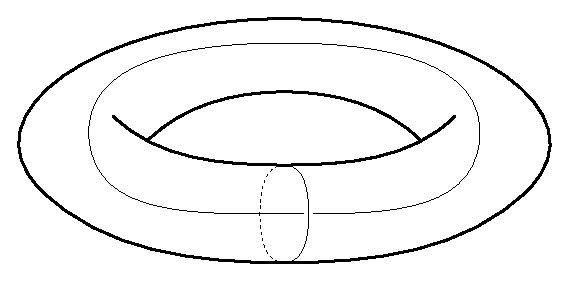
\includegraphics{figs/chain_link_fence_knot_on_torus.eps}
            \caption{Chain-Link Fence on a Torus}
            \label{fig:chain_link_fence_on_torus}
        \end{figure}
    \end{frame}
    \begin{frame}{The Knot Graph}
        The knot graph for this virtual knot is shown below on the flat torus.
        \begin{figure}
            \centering
            \includegraphics{figs/knot_graph_chain_link_fence_001.eps}
            \caption{Knot Graph for the Chain-Link Fence}
            \label{fig:chain_link_fence_knot_graph}
        \end{figure}
    \end{frame}
    \begin{frame}{Medial Graph}
        The knot graph is not the only way to turn a knot into a graph,
        and it's not the best way either. This shows that every knot
        corresponds to a graph, but we can't go the other way around.
        The knot graph must be a 4-regular multigraph, and there are plenty of
        graphs lacking these features.
    \end{frame}
    \begin{frame}{Medial Graph}
    	\begin{definition}[Medial Graph]
        	Let $G$ be a planar graph embedded in the plane in with some planar embedding.
        	\pause Then the \textit{medial graph of $G$ with respect to the embedding},
        	denoted by $\Gamma(G)$, is the graph whose vertex set is the edge set of $G$, and two vertices
        	in $\Gamma(G)$ are adjacent if, as edges of $G$, they are consecutive edges for some
        	(possibly unbounded) face of $G$. \pause (A \textit{face} of $G$ is a connected region enclosed
        	by some number of edges.)
        \end{definition}
    \end{frame}
\begin{frame}{Example of a Planar Graph and Associated Medial Graph}
	\scalebox{.7}{
	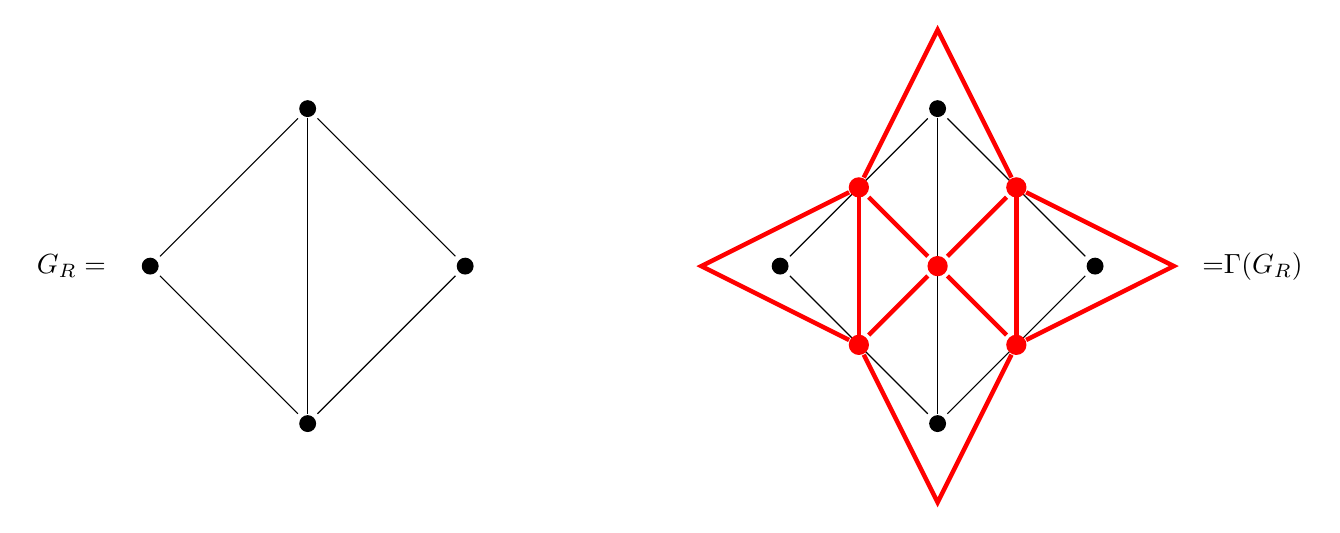
\begin{tikzpicture}
	\node (G) at (-1, 2) {$G_R =$};
	\node (A) at (2,0) {};
	\node (B) at (0,2) {};
	\node (C) at (4,2) {};
	\node (D) at (2,4) {};
	\draw[fill] (A) circle (.1cm);
	\draw[fill] (B) circle (.1cm);
	\draw[fill] (C) circle (.1cm);
	\draw[fill] (D) circle (.1cm);
	\draw[-] (A) -- (D);
	\draw[-] (A) -- (C);
	\draw[-] (A) -- (B);
%	\draw[-] (B) -- (C);
	\draw[-] (B) -- (D);
	\draw[-] (C) -- (D);
	

	\node (G2) at (14, 2) {=$\Gamma(G_R)$};
	\node (A2) at (10,0) {};
	\node (B2) at (8,2) {};
	\node (C2) at (12,2) {};
	\node (D2) at (10,4) {};
	\node (E1) at (9,3) {};
	\node (E2) at (10,2) {};
	\node (E3) at (11,3) {};
	\node (E4) at (9,1) {};
	\node (E5) at (11,1) {};
	\draw[fill] (A2) circle (.1cm);
	\draw[fill] (B2) circle (.1cm);
	\draw[fill] (C2) circle (.1cm);
	\draw[fill] (D2) circle (.1cm);
	\draw[-] (A2) -- (D2);
	\draw[-] (A2) -- (C2);
	\draw[-] (A2) -- (B2);
%	\draw[-] (B) -- (C);
	\draw[-] (B2) -- (D2);
	\draw[-] (C2) -- (D2);
	\draw[fill, color = red, ultra thick] (E1) circle (.1cm);
	\draw[fill, color = red, ultra thick] (E2) circle (.1cm);
	\draw[fill, color = red, ultra thick] (E3) circle (.1cm);
	\draw[fill, color = red, ultra thick] (E4) circle (.1cm);
	\draw[fill, color = red, ultra thick] (E5) circle (.1cm);
	\draw[-, color = red, ultra thick] (E2) -- (E1);
	\draw[-, color = red, ultra thick] (E2) -- (E3);
	\draw[-, color = red, ultra thick] (E2) -- (E4);
	\draw[-, color = red, ultra thick] (E2) -- (E5);
	%\draw[-, color = red] (E1) -- (E3);
	%\draw[-, color = red] (E4) -- (E5);
	\draw[-, color = red, ultra thick] (E4) -- (E1);
	\draw[-, color = red, ultra thick] (E5) -- (E3);
	\draw[-,red, ultra thick] (E4)-- (10,-1) --(E5); 
	\draw[-,red, ultra thick] (E4)-- (7,2)--(E1); 
	\draw[-,red, ultra thick] (E1)--(10,5)--(E3); 
	\draw[-,red, ultra thick] (E3) -- (13,2) --(E5); 

\end{tikzpicture}
}
\end{frame}
\begin{frame}{How to Turn a Medial Graph into a Link}
	\begin{itemize}
	\pause\item Pick some arbitrary vertex $v$ of the medial graph.
	\pause\item Pick some arbitrary edge, $(u,v)$, that connects $v$ to some other vertex $u$.
	\pause\item The next edge which will be part of the link is the edge which does not follow or proceed the edge $(u,v)$ in a clockwise orientation around $u$.  This edge well-defined since the medial graph is 4-regular. 
	\pause\item  Then repeat this process until an edge is repeated. The collection of edges determined by this will be the link component.
\end{itemize} 
\end{frame}
\begin{frame}{Example of Medial Link Diagrams}
\centering
\scalebox{1.2}{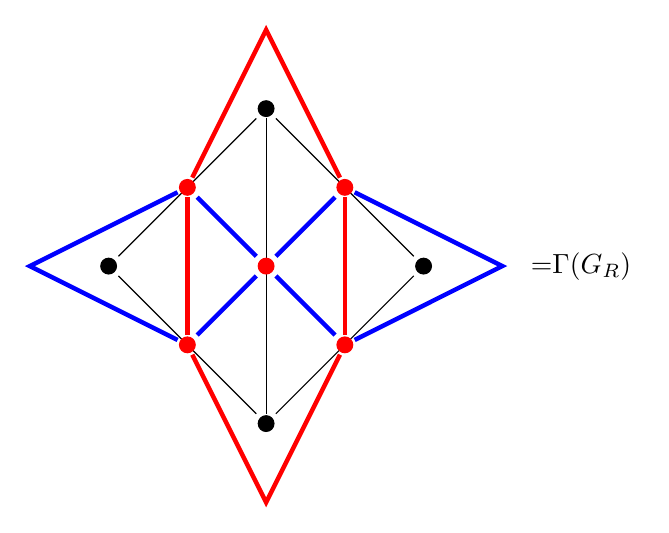
\begin{tikzpicture}
	\node (G2) at (6, 2) {=$\Gamma(G_R)$};
	\node (A2) at (2,0) {};
	\node (B2) at (0,2) {};
	\node (C2) at (4,2) {};
	\node (D2) at (2,4) {};
	\node (E1) at (1,3) {};
	\node (E2) at (2,2) {};
	\node (E3) at (3,3) {};
	\node (E4) at (1,1) {};
	\node (E5) at (3,1) {};
	\draw[fill] (A2) circle (.1cm);
	\draw[fill] (B2) circle (.1cm);
	\draw[fill] (C2) circle (.1cm);
	\draw[fill] (D2) circle (.1cm);
	\draw[-] (A2) -- (D2);
	\draw[-] (A2) -- (C2);
	\draw[-] (A2) -- (B2);
%	\draw[-] (B) -- (C);
	\draw[-] (B2) -- (D2);
	\draw[-] (C2) -- (D2);
	\draw[fill, color = red] (E1) circle (.1cm);
	\draw[fill, color = red] (E2) circle (.1cm);
	\draw[fill, color = red] (E3) circle (.1cm);
	\draw[fill, color = red] (E4) circle (.1cm);
	\draw[fill, color = red] (E5) circle (.1cm);
	\draw[-, color = blue, ultra thick] (E2) -- (E1);
	\draw[-, color = blue, ultra thick] (E2) -- (E3);
	\draw[-, color = blue, ultra thick] (E2) -- (E4);
	\draw[-, color = blue, ultra thick] (E2) -- (E5);
%	\draw[-, color = red] (E1) -- (E3);
%	\draw[-, color = red] (E4) -- (E5);
	\draw[-, color = red, ultra thick] (E4) -- (E1);
	\draw[-, color = red, ultra thick] (E5) -- (E3);
	\draw[-,red, ultra thick](E4)-- (2,-1)-- (E5); 
	\draw[-,blue, ultra thick] (E4)-- (-1,2) --(E1); 
	\draw[-,red, ultra thick] (E1) --(2,5)-- (E3); 
	\draw[-,blue, ultra thick] (E3) --(5,2) --(E5); 
\end{tikzpicture}
}	
\end{frame}
\begin{frame}{Checkerboard Coloring}
	\begin{definition}[Checkerboard Coloring of a Link]
	Let $l$ be an arbitrary link with link projection $L$. Then without loss of generality, assume that the unbounded region of $L$ is considered unshaded.
\pause For each region $R$, if $R$ shares an edge along its boundary with the boundary of an unshaded region, then $R$ is considered shaded, and vice versa. 
\pause A drawing of $L$ with regions shaded according to this process is called a \textit{checkerboard} coloring of a link.
\end{definition} 
\end{frame}
\begin{frame}{Example of a Medial Link Diagram with the Checkerboard Coloring}
\centering
	\scalebox{1.2}{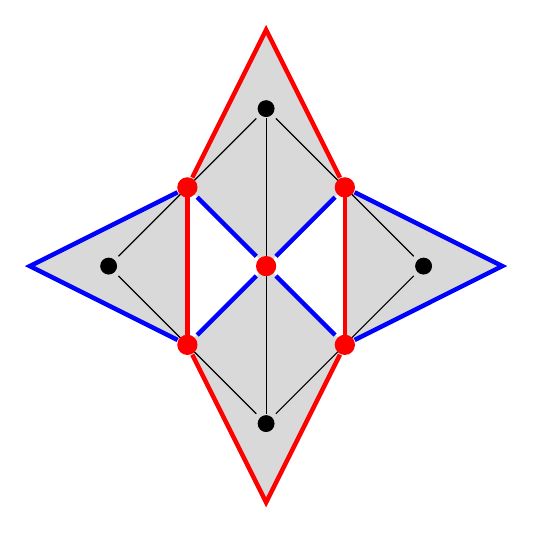
\begin{tikzpicture}
	\node (A2) at (2,0) {};
	\node (B2) at (0,2) {};
	\node (C2) at (4,2) {};
	\node (D2) at (2,4) {};
	\node (E1) at (1,3) {};
	\node (E2) at (2,2) {};
	\node (E3) at (3,3) {};
	\node (E4) at (1,1) {};
	\node (E5) at (3,1) {};
	\fill[gray!30] (-1,2) -- (1,3)--(1,1);
	\fill[gray!30] (5,2) -- (3,3)--(3,1);
	\fill[gray!30] (2,-1) -- (1,1)--(2,2)--(3,1);
	\fill[gray!30] (2,5) -- (3,3)--(2,2)--(1,3);
	\draw[fill] (A2) circle (.1cm);
	\draw[fill] (B2) circle (.1cm);
	\draw[fill] (C2) circle (.1cm);
	\draw[fill] (D2) circle (.1cm);
	\draw[-] (A2) -- (D2);
	\draw[-] (A2) -- (C2);
	\draw[-] (A2) -- (B2);
%	\draw[-] (B) -- (C);
	\draw[-] (B2) -- (D2);
	\draw[-] (C2) -- (D2);
	\draw[fill, color = red, ultra thick] (E1) circle (.1cm);
	\draw[fill, color = red, ultra thick] (E2) circle (.1cm);
	\draw[fill, color = red, ultra thick] (E3) circle (.1cm);
	\draw[fill, color = red, ultra thick] (E4) circle (.1cm);
	\draw[fill, color = red, ultra thick] (E5) circle (.1cm);
	\draw[-, color = blue, ultra thick] (E2) -- (E1);
	\draw[-, color = blue, ultra thick] (E2) -- (E3);
	\draw[-, color = blue, ultra thick] (E2) -- (E4);
	\draw[-, color = blue, ultra thick] (E2) -- (E5);
%	\draw[-, color = red] (E1) -- (E3);
%	\draw[-, color = red] (E4) -- (E5);
	\draw[-, color = red, ultra thick] (E4) -- (E1);
	\draw[-, color = red, ultra thick] (E5) -- (E3);
	\draw[-,red, ultra thick](E4)-- (2,-1)-- (E5); 
	\draw[-,blue, ultra thick] (E4)-- (-1,2) --(E1); 
	\draw[-,red, ultra thick] (E1) --(2,5)-- (E3); 
	\draw[-,blue, ultra thick] (E3) --(5,2) --(E5); 
	\end{tikzpicture}
}
\end{frame}
\begin{frame}{Over-Under Information by Signings}
		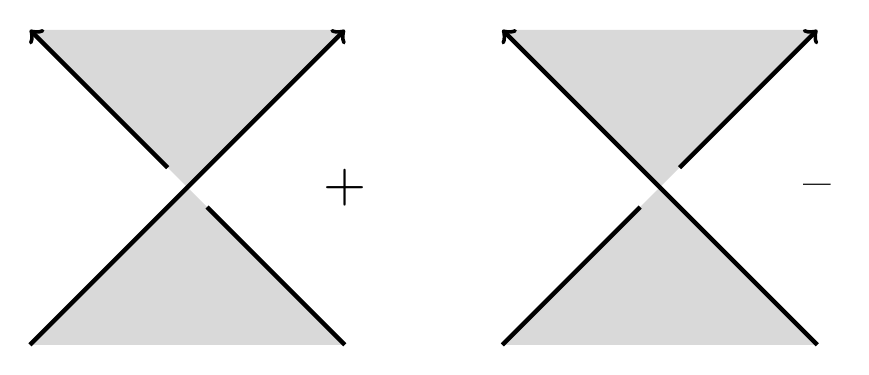
\begin{tikzpicture}
	\fill[gray!30] (0,0) --(2,2) -- (4,0);
		\fill[gray!30] (4,4) --(2,2) -- (0,4);
		\draw[->,ultra thick] (0,0) -- (4,4);
		%\draw[-, ultra thick] (0,4) -- (4,0);
		\draw[<-, ultra thick] (0,4) -- (1.75,2.25);
		\draw[-, ultra thick] (2.25,1.75) -- (4,0);
		\node (+) at (4,2){\scalebox{2}{+}};	
			\fill[gray!30] (6,0) --(8,2) -- (10,0);
		\fill[gray!30] (10,4) --(8,2) -- (6,4);
		\draw[-,ultra thick] (6,0) -- (7.75,1.75);
		\draw[<-, ultra thick] (6,4) -- (10,0);
		%\draw[-, ultra thick] (0,4) -- (1.75,2.25); 
		\draw[->, ultra thick] (8.25,2.25) -- (10,4);
		\node (-) at (10,2){\scalebox{2}{--}};
	\end{tikzpicture}
\end{frame}
\begin{frame}{Example of Medial Link Construction for a Signed Graph}
	\begin{center}
	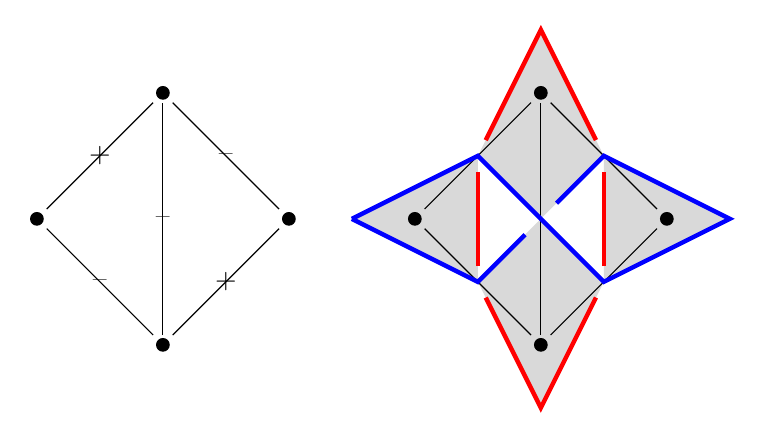
\begin{tikzpicture}[scale = .8]
	\node (A2) at (2,0) {};
	\node (B2) at (0,2) {};
	\node (C2) at (4,2) {};
	\node (D2) at (2,4) {};
	\node (E1) at (1,3) {+};
	\node (E2) at (2,2) {--};
	\node (E3) at (3,3) {--};
	\node (E4) at (1,1) {--};
	\node (E5) at (3,1) {+};
% 	\fill[gray!30] (-1,2) -- (1,3)--(1,1);
% 	\fill[gray!30] (5,2) -- (3,3)--(3,1);
% 	\fill[gray!30] (2,-1) -- (1,1)--(2,2)--(3,1);
% 	\fill[gray!30] (2,5) -- (3,3)--(2,2)--(1,3);
	\draw[fill] (A2) circle (.1cm);
	\draw[fill] (B2) circle (.1cm);
	\draw[fill] (C2) circle (.1cm);
	\draw[fill] (D2) circle (.1cm);
	\draw[-] (A2) -- (D2);
	\draw[-] (A2) -- (C2);
	\draw[-] (A2) -- (B2);
%	\draw[-] (B) -- (C);
	\draw[-] (B2) -- (D2);
	\draw[-] (C2) -- (D2);
% 	\draw[fill, color = red, ultra thick] (E1) circle (.1cm);
% 	\draw[fill, color = red, ultra thick] (E2) circle (.1cm);
% 	\draw[fill, color = red, ultra thick] (E3) circle (.1cm);
% 	\draw[fill, color = red, ultra thick] (E4) circle (.1cm);
% 	\draw[fill, color = red, ultra thick] (E5) circle (.1cm);
% 	\draw[-, color = blue, ultra thick] (E2) -- (E1);
% 	\draw[-, color = blue, ultra thick] (E2) -- (E3);
% 	\draw[-, color = blue, ultra thick] (E2) -- (E4);
% 	\draw[-, color = blue, ultra thick] (E2) -- (E5);
% %	\draw[-, color = red] (E1) -- (E3);
% %	\draw[-, color = red] (E4) -- (E5);
% 	\draw[-, color = red, ultra thick] (E4) -- (E1);
% 	\draw[-, color = red, ultra thick] (E5) -- (E3);
% 	\draw[-,red, ultra thick](E4)-- (2,-1)-- (E5); 
% 	\draw[-,blue, ultra thick] (E4)-- (-1,2) --(E1); 
% 	\draw[-,red, ultra thick] (E1) --(2,5)-- (E3); 
% 	\draw[-,blue, ultra thick] (E3) --(5,2) --(E5); 
	\begin{scope}[shift = {(6,0)}]
	\node (A2) at (2,0) {};
	\node (B2) at (0,2) {};
	\node (C2) at (4,2) {};
	\node (D2) at (2,4) {};
%	\node (E1) at (1,3) {};
%	\node (E2) at (2,2) {};
%	\node (E3) at (3,3) {};
%	\node (E4) at (1,1) {};
%	\node (E5) at (3,1) {};
	\fill[gray!30] (-1,2) -- (1,3)--(1,1);
	\fill[gray!30] (5,2) -- (3,3)--(3,1);
	\fill[gray!30] (2,-1) -- (1,1)--(2,2)--(3,1);
	\fill[gray!30] (2,5) -- (3,3)--(2,2)--(1,3);
	\draw[fill] (A2) circle (.1cm);
	\draw[fill] (B2) circle (.1cm);
	\draw[fill] (C2) circle (.1cm);
	\draw[fill] (D2) circle (.1cm);
	\draw[-] (A2) -- (D2);
	\draw[-] (A2) -- (C2);
	\draw[-] (A2) -- (B2);
%	\draw[-] (B) -- (C);
	\draw[-] (B2) -- (D2);
	\draw[-] (C2) -- (D2);
%	\draw[fill, color = red, ultra thick] (E1) circle (.1cm);
%	\draw[fill, color = red, ultra thick] (E2) circle (.1cm);
%	\draw[fill, color = red, ultra thick] (E3) circle (.1cm);
%	\draw[fill, color = red, ultra thick] (E4) circle (.1cm);
%	\draw[fill, color = red, ultra thick] (E5) circle (.1cm);
%	\draw[-, color = blue, thick] (1,3) -- (2,2);
%	\draw[-, color = blue, ultra thick] (2,2) -- (3,3);
%	\draw[-, color = blue, ultra thick] (2,2) -- (1,1);
%	\draw[-, color = blue, ultra thick] (2,2) -- (3,1);
%	\draw[-, color = red] (E1) -- (E3);
%	\draw[-, color = red] (E4) -- (E5);
%	\draw[-, color = red] (1,1) -- (1,3);
%	\draw[-, color = red] (3,1) -- (3,3);
%	\draw[-,red, ultra thick](1,1)-- (2,-1)-- (3,1); 
%	\draw[-,blue, ultra thick] (1,1)-- (-1,2) --(1,3); 
%	\draw[-,red, ultra thick] (1,3) --(2,5)-- (3,3); 
%	\draw[-,blue, ultra thick] (3,3) --(5,2) --(3,1); 
\draw[-,blue, ultra thick] (-1,2) -- (1,3) -- (3,1) -- (5,2) -- (3,3)-- (2.25, 2.25);
\draw[-,blue, ultra thick] (1.75,1.75) -- (1,1) -- (-1,2);
\draw[-, red, ultra thick] (2.875,.75) --(2,-1) -- (1.125, .75);
\draw[-, red, ultra thick] (2.875,3.25) --(2,5) -- (1.125, 3.25);
\draw[-, red, ultra thick] (1, 1.25) -- (1, 2.75);
\draw[-, red, ultra thick] (3, 1.25) -- (3, 2.75);
	\end{scope}
	\end{tikzpicture}
\end{center}
\end{frame}
    \begin{frame}{Dual Graph}
        Given a planar graph, we can draw it in the plane without crossings.
        This will result in several regions of the plane being enclosed by
        the edges of the graph. These are called the \textit{faces} of the
        graph. How many faces are there in $K_{4}$?
        \begin{figure}
            \centering
            \includegraphics{figs/complete_graph_K4_planar_straight_lines.eps}
            \caption{$K_{4}$}
            \label{fig:K_4}
        \end{figure}
    \end{frame}
    \begin{frame}{Dual Graph}
        It may be tempting to say that there are 3 faces, but we should convince
        ourselves that there are 4. There are the 3 faces enclosed by the triangles,
        but there is also the entire \textit{outside}. It is weird to think of this
        as a face, but the reasoning is a lot clearer if we draw $K_{4}$ on a
        \textit{sphere}.
        \begin{figure}
            \centering
            \includegraphics{figs/complete_graph_k4_faces.eps}
            \caption{The faces of $K_{4}$}
            \label{fig:k4_faces}
        \end{figure}
    \end{frame}
    \begin{frame}{Dual Graph}
        On a sphere, the outside face is indeed a closed region, and doesn't
        \textit{go off to infinity}. Because of this, we label the outside as a
        face for any planar graph.
        \begin{figure}
            \centering
            \includegraphics{figs/complete_graph_k4_on_sphere.eps}
            \caption{$K_{4}$ on a sphere}
            \label{fig:k4_on_sphere}
        \end{figure}
    \end{frame}
    \begin{frame}{Dual Graph}
        The \textit{dual graph} of a planar graph is obtained by placing
        a vertex at each face, and connecting two vertices with an edge if
        the original faces share an edge. Below is the dual graph for $K_{4}$.
        Looking closely, we see the dual is also $K_{4}$. That is,
        $K_{4}$ is \textit{self-dual}.
        \begin{figure}
            \centering
            \includegraphics{figs/complete_graph_k4_dual_graph.eps}
            \caption{$K_{4}$ dual graph}
            \label{fig:k4_dual}
        \end{figure}
    \end{frame}
    \begin{frame}{Dual Graph}
        The dual graph of a simple planar graph does not need to be simple.
        Let's look at $K_{3}$. There 2 faces, the \textit{inside} and
        \textit{outside}, and hence 2 vertices. Moreover, these faces
        share 3 edges, so there are 3 edges in the dual graph. It is a
        multigraph.
        \begin{figure}
            \centering
            \begin{subfigure}[b]{0.49\textwidth}
                \centering
                \includegraphics{figs/complete_graph_k3_dual_graph_001.eps}
            \end{subfigure}
            \begin{subfigure}[b]{0.49\textwidth}
                \centering
                \includegraphics{figs/complete_graph_k3_dual_graph_002.eps}
            \end{subfigure}
            \caption{$K_{3}$ dual graph}
            \label{fig:k3_dual}
        \end{figure}
    \end{frame}
    \begin{frame}{Dual Graph}
        What happens if we take the dual of the dual of a graph? That is,
        we start with a planar graph $G$, get a dual graph $G'$, and then look
        at the dual graph of $G'$, call it $G''$. Is this a new graph? It turns
        out $G$ and $G''$ are the \textit{same} graph.
    \end{frame}
    \begin{frame}{Dual Graph}
        What about \textit{non-planar} graphs? Can we make sense of the dual graph
        for these? We can if we embed them onto higher genus surfaces. Figuring out
        the faces can be very tricky. Let's look at one of the simplest virtual
        knots, the 1 crossing link.
        \begin{figure}
            \centering
            \includegraphics{figs/one_crossing_link_on_torus.eps}
            \caption{1-Crossing link on a torus}
            \label{fig:one_crossing_link_on_torus}
        \end{figure}
    \end{frame}
    \begin{frame}{Dual Graph}
        We can also look at a 3D version of this, if it helps.
        \begin{figure}
            \centering
            \includegraphics{figs/one_crossing_link_on_torus_3d.eps}
            \caption{1-Crossing link on a torus}
            \label{fig:one_crossing_link_on_torus_3d}
        \end{figure}
    \end{frame}
    \begin{frame}{Dual Graph}
        We now want to look at the knot graph of this virtual link.
        The link is drawn on the flat torus below, and the graph is given
        next to it. Since there's only 1 crossing, it doesn't matter which way
        we orient the links.
        \begin{figure}
            \centering
            \begin{subfigure}[b]{0.49\textwidth}
                \includegraphics{figs/one_crossing_link_on_flat_torus.eps}
                \caption{1-Crossing link on flat torus}
                \label{fig:one_crossing_link_flat_torus}
            \end{subfigure}
            \begin{subfigure}[b]{0.49\textwidth}
                \includegraphics{figs/knot_graph_one_crossing_link.eps}
                \caption{1-Crossing graph on flat torus}
                \label{fig:one_crossing_graph_flat_torus}
            \end{subfigure}
        \end{figure}
    \end{frame}
    \begin{frame}{Dual Graph}
        How many faces are there for this graph? 4? 2? 1?
        Let's look at this graph through the eyes of Pac-Man and see
        what we find.
        \begin{figure}
            \centering
            \includegraphics{figs/knot_graph_one_crossing_link_plane.pdf}
            \caption{Knot Graph for 1-crossing link on the plane.}
            \label{fig:knot_graph_one_crossing_link_plane}
        \end{figure}
    \end{frame}
    \begin{frame}{Dual Graph}
        The dual graph has \textit{one} face. The face touches itself
        4 times to the east, west, north, and south. The so dual graph
        has 1 vertex and 4 edges.
        \begin{figure}
            \centering
            \includegraphics{figs/dual_graph_one_crossing_torus_link.eps}
            \caption{Dual graph for the knot graph of the 1-crossing link}
            \label{fig:dual_graph_one_crossing_torus_link}
        \end{figure}
    \end{frame}
    \begin{frame}{Dual Graph}
        Try to find the faces and edges for $K_{5}$.
        \begin{figure}
            \centering
            \includegraphics[scale=0.35]{figs/dual_graph_k5_flat_torus.eps}
            \caption{$K_{5}$ dual graph}
            \label{fig:k5_dual}
        \end{figure}
    \end{frame}
    \begin{frame}{Dual Graph}
        Try to find the faces and edges for $K_{3,3}$.
        \begin{figure}
            \centering
            \includegraphics[scale=0.35]{figs/dual_graph_k3_3_on_flat_torus.eps}
            \caption{$K_{3,3}$ dual graph}
            \label{fig:k3_3_dual}
        \end{figure}
    \end{frame}
    \begin{frame}{Dual Graph}
        We'll end with an exercise in finding faces for graphs on
        the torus. Before doing this, it helps to mention the torus can
        also be represented by a \textit{hexagon}. See below.
        \begin{figure}
            \centering
            \includegraphics[scale=0.6]{figs/hexagon_as_torus.png}
            \caption{Hexagon to Torus}
            \label{fig:hexagon_as_torus}
        \end{figure}
    \end{frame}
    \begin{frame}{Dual Graph}
        Try to find the dual graph of $K_{7}$ on the torus. You can use
        the square or hexagonal representation of the torus.
        \begin{figure}
            \centering
            \includegraphics{figs/complete_graph_k7.eps}
            \caption{$K_{7}$}
            \label{fig:k7}
        \end{figure}
    \end{frame}
    \begin{frame}{Solution}
        \begin{figure}
            \centering
            \includegraphics[scale=0.2]{figs/k7_dual_graph_torus.png}
            \caption{Dual Graph for $K_{7}$}
            \label{fig:k7_dual_graph_torus}
        \end{figure}
    \end{frame}
\end{document}